\clearpage

\begin{figure}
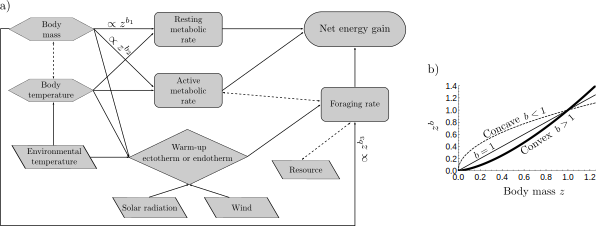
\includegraphics[width=\textwidth]{fig1}
\caption{
    \setstretch{\stretchby}
    % E: For a figure to have multiple panels, the panels need to relate to one another.  Could (a) include, say, notes on the lines that depict power laws?
    Model components.
    (a) Unidirectional solid lines show one component affecting another.
    Bidirectional dashed lines show a correlation or indirect link between the two components.
    Input variables are denoted by hexagons for intrinsic variables and the non-rhomboid parallelograms for environmental variables.
    The main processes are denoted by rounded rectangles (metabolic and foraging rates) and the rhombus means that warm-up needs to be completed before foraging.
    (b) Power law functions of body mass, $z$, are used throughout the model for the relationship between body mass and metabolic and foraging rates in (a).
    The expression $z^b$ is concave when $0 < b < 1$ and convex when $b > 1$.
}
\label{fig1}
\end{figure}

\begin{figure}
\includegraphics[width=\textwidth]{fig2}
\caption{
    \setstretch{\stretchby}
    Scenarios whereby thermal performance does or does not peak at intermediate body mass.
    In each panel, dashed, thin, and thick lines depict different foraging rate exponents ($b_3 = 0.5,\ 0.8,\ \text{and } 1.25$, respectively).
    ``Standard'' extrinsic parameter values are
    resource quantity $R = 500$ (defined only when the resource amount is fixed; panels a,b,e,f),
    resource quality $\rho = 12$,
    foraging time $\tau_f = 45 \text{ min}$ (defined only when foraging time is fixed; panels c,d,g,h),
    and environmental temperature $T_e = 15^\circ C$.
    Intrinsic parameter values for active metabolic rate are $a_2 = 20 a_1 \text{ and } b_2 = 0.75$ for ``standard'' (panels a--d), and $a_2 = 30 a_1 \text{ and } b_2  = 1.25$ for ``higher'' (panels e--h).
    Additional parameter values and measurement units are provided in \cref{table:table1}.
}
\label{fig2}
\end{figure}

\begin{figure}
\centering \includegraphics[width=0.9\textwidth]{fig3}
\caption{
    \setstretch{\stretchby}
	Warm-up for ectotherms and endotherms.
	a) Lowest temperature that allows the completion of warm-up, as a function of body mass.
	The individual is given a maximum of six hours to complete warm-up.
    Thick, thin, and dashed lines represent endotherms with laminar convection, ectotherms with laminar convection, and ectotherms with free convection, respectively.
    Solar radiation is 1/4 the value at 30$^\circ$ latitude during equinox, and the convection factor is $K_2 = 0.1$.
    b) Duration of warm-up for endotherms (thick lines) and ectotherms (dashed lines) as a function of body mass and temperature, for free convection.  % E: correct to add "free convection"?
    Solar radiation is not reduced and $K_2 = 1$.
    For a) and b), wind speed $u = 1$, contraction frequency constant $a_w = 1.25$, and other parameter values and units are in \cref{table:table1}.
	% Fixed parameter values: default conductance $K_1 = 0.05 \, c_p, r_3 = 0.5$.
}
\label{fig3}
\end{figure}
%
\begin{figure}
\centering \includegraphics[width=0.9\textwidth]{fig4}
\caption{
    \setstretch{\stretchby}
    Effect of warm-up on thermal performance for small (thin lines, $z = 0.5$) and large (thick lines, $z = 2$) individuals under free convection.
    Warm-up starts half an hour after sunrise with a total foraging time $\tau_f = 1$.
    Parameter values are $\rho = 24,\ a_2 = 10,\ a_1 = ??,\ b_1 = b_2 = b_3 = 0.75$, and otherwise as in \cref{table:table1}. % FIXME: need the value for a_1
}
\label{fig4}
\end{figure}

\clearpage

\begin{figure}
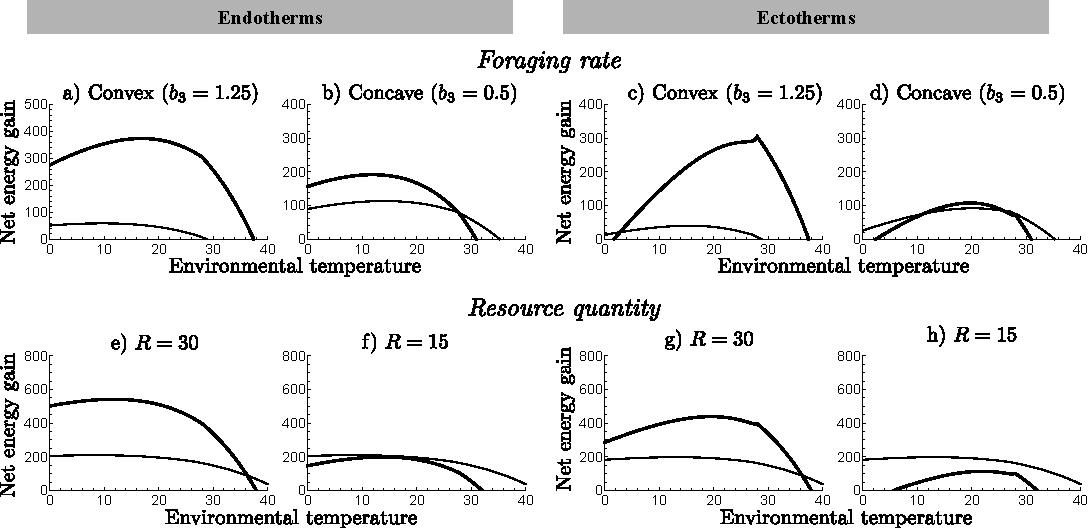
\includegraphics[width=\textwidth]{fig5}
\caption{
    \setstretch{\stretchby}
	Foraging rate and resource quantity affect thermal performance curves.
	Results are shown for small (thin lines, $z = 0.5$ in a--d, $z = 0.2$ in e--h) and large (thick lines, $z = 2$) individuals.
	Other assumptions are free convection, warm-up starting half an hour after sunrise, $\rho = 24,\ a_2 = 10,\ a_1 = 1, b_1 = b_2 = 0.75 $.
    For a--d, foraging time is $\tau_f = 1$.
    For e--h, $b_3 = 0.75$.
    Units and other parameter values are in \cref{table:table1}.
}
\label{fig5}
\end{figure}
